\documentclass[a4j]{jarticle}

\usepackage[dvipdfmx]{graphicx}
\usepackage{url}
\usepackage{here}
%\usepackage{listings}
\usepackage{amsmath,amssymb}
\usepackage[dvipdfmx]{color}

\setlength{\headsep}{-5mm}
\setlength{\oddsidemargin}{0mm}
\setlength{\textwidth}{165mm}
\setlength{\textheight}{230mm}
\setlength{\footskip}{20mm}

\title{
\vspace{30mm}
{\bf 子育て支援システム}
\\
\vspace{5mm}
{\bf 内部設計書v1\\
}
\vspace{120mm}
}

\author{
\vspace{5mm}
チーム名 007\\
\vspace{5mm}
}


\begin{document}
\maketitle
\tableofcontents
\newpage

\section{モジュール設計書}
\subsection{フロー図}
本システムのモジュール構成をフロー図として図\ref{functionselection}、図\ref{initialsetting}に示します。モジュール構成において各図形が何を意味するか図\ref{sample}に示してあります。

\begin{figure}[H]
    \begin{center}
    \resizebox{8cm}{!}{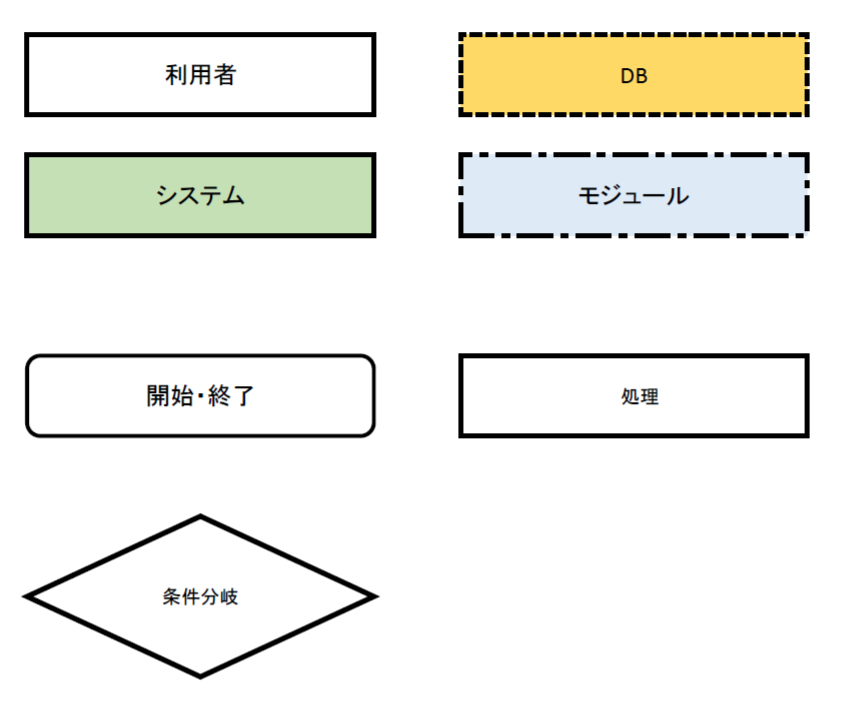
\includegraphics {sample.png}}
    \caption {見本のイメージ}
    \label{sample}
    \end{center}
\end{figure}

図\ref{sample}より、無色の図が「利用者側の操作」、緑色の図が「システム側の動作」、点線かつ黄色の図が「データベース側の動作」、かつ水色の図が「モジュール」を意味します。また、角の丸い四角形は「各モジュールの開始時・終了時の処理」、四角形は「各モジュールの中の処理」、ひし形は「条件分岐」を意味します。

\begin{figure}[H]
    \begin{center}
    \resizebox{16.5cm}{!}{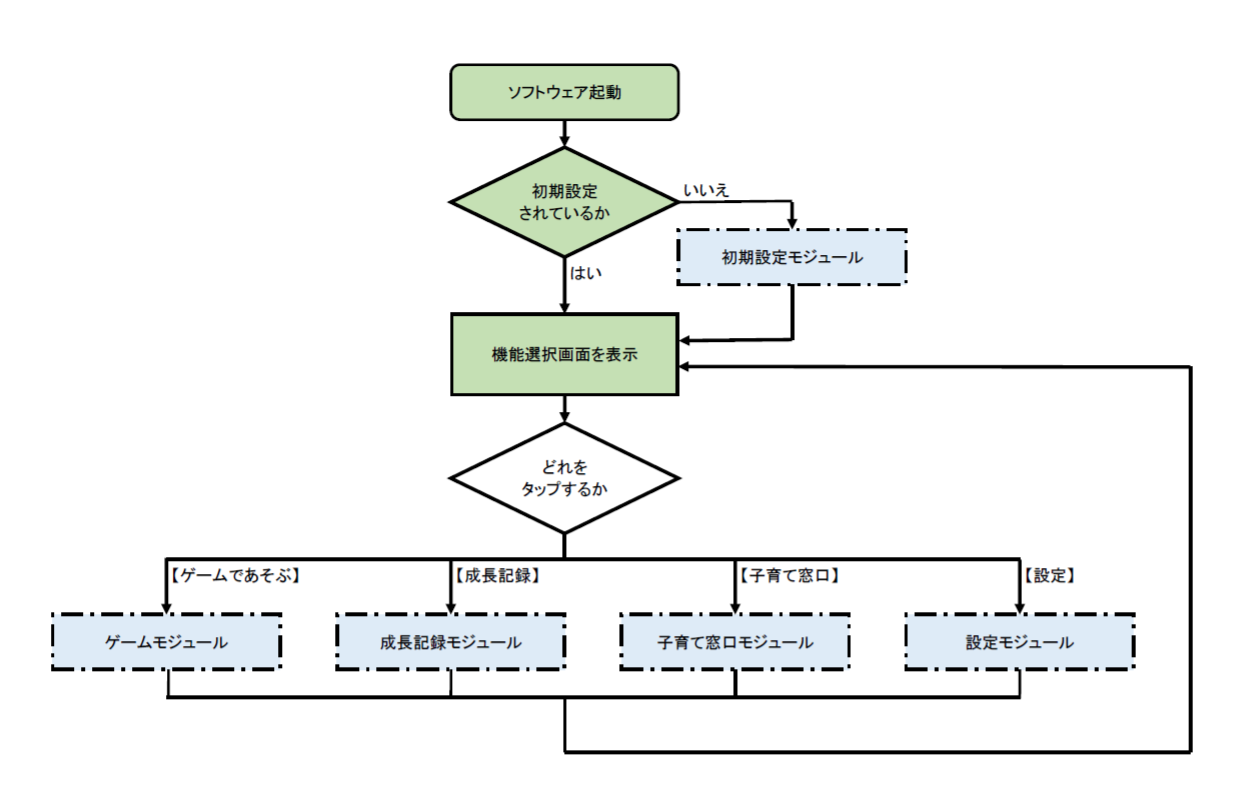
\includegraphics {functionselection.png}}
    \caption {機能選択モジュールのイメージ}
    \label{functionselection}
    \end{center}
\end{figure}

\begin{figure}[H]
    \begin{center}
    \resizebox{16.5cm}{!}{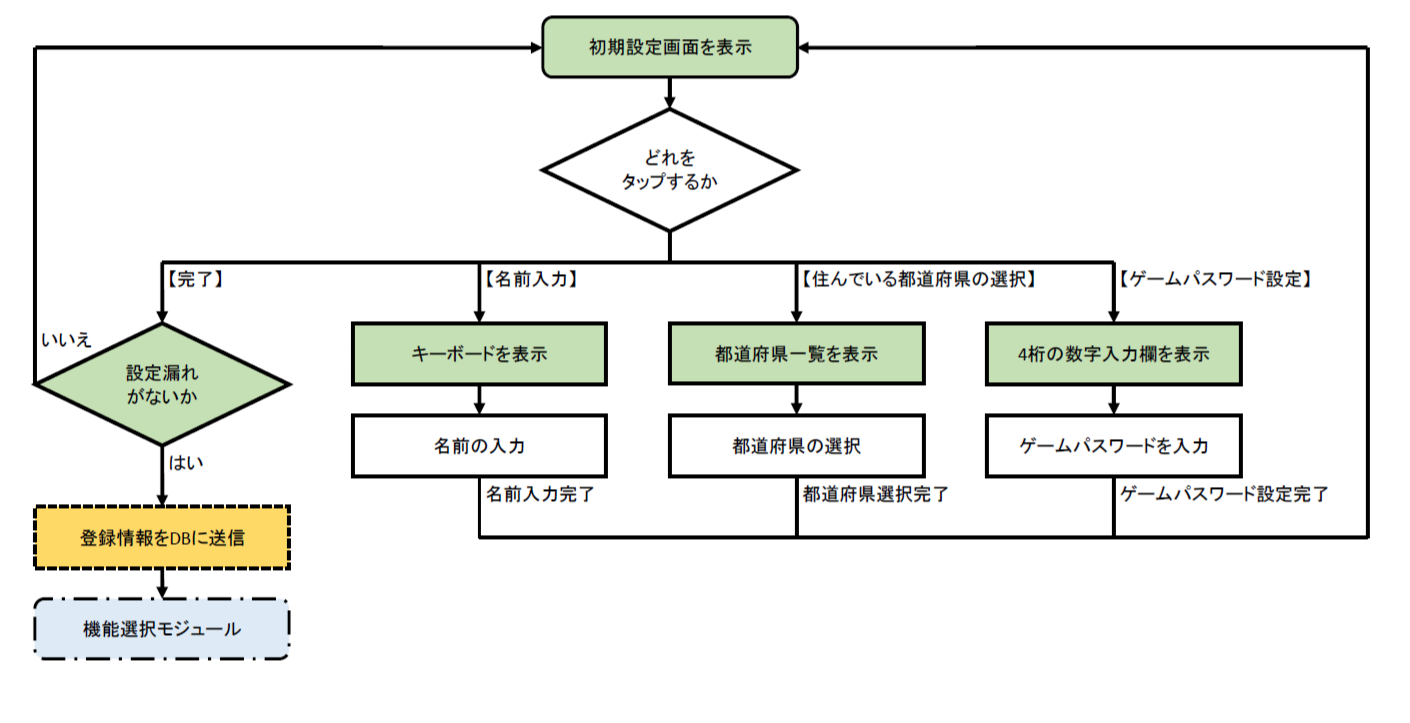
\includegraphics {initialsetting.png}}
    \caption {初期設定モジュールのイメージ}
    \label{initialsetting}
    \end{center}
\end{figure}

\subsection{モジュール仕様}
各モジュールの具体的な説明を行う。

\subsubsection{機能選択モジュール}
〔概要〕
本システムを起動してから各機能選択を行うまでの流れを示しています。

〔処理フロー〕
\begin{itemize}
\item 本システムを起動した際に、初期設定が行われていればそのまま機能選択画面を表示させます。初期設定が行われていない場合は初期設定モジュールを呼び出します。

\item 【ゲームであそぶボタン】タップすることでゲームモジュールを呼び出します。

\item 【成長記録ボタン】をタップすることで成長記録モジュールを呼び出します。

\item 【子育て窓口ボタン】をタップすることで子育て窓口モジュールを呼び出しします。

\item 【設定ボタン】をタップすることで設定モジュールを呼び出しします。

\item 機能選択画面から呼び出される各モジュールにおいて【もどるボタン】をタップすることで、機能選択画面に戻ります。
\end{itemize}

\subsubsection{初期設定モジュール}
〔概要〕
本システムを初めて利用する場合、最初に行う初期設定機能です。

〔処理フロー〕
\begin{itemize}
\item 【名前(ニックネーム)の入力欄】をタップすることで画面下にキーボードが表示され、名前入力を行えるようになります。

\item 【居住地域の選択欄の矩形領域】をタップすることで47都道府県をタップして選択できるドロップダウンリストを表示させ、住んでいる地域設定が行えるようになります。

\item 【ゲームのパスワードの入力欄】をタップすることでキーボードを表示させ、ゲーム画面から機能選択画面に戻るためのパスワードとして、4桁の数字が入力できるようになります。

\item 【完了ボタン】をタップすることで初期設定が全て行われているか判定を行い、設定漏れがなければデータベースに初期設定情報を登録して機能選択画面に遷移します。設定漏れが見つかれば再び初期設定画面に戻り、設定漏れを埋めることになります。
\end{itemize}



\end{document}
